%-briefly recaps the project purposes and goals,
\documentclass[onecolumn, draftclsnofoot,10pt, compsoc]{IEEEtran}
\usepackage{graphicx}
\usepackage{url}
\usepackage{setspace}
\usepackage{cite}
\usepackage{tabularx}
%\usepackage{pgfgantt}
\usepackage{listings}
\usepackage{longtable}
\usepackage{minted}

\usepackage{geometry}
\geometry{textheight=9.5in, textwidth=7in}



% 1. Fill in these details
\def \CapstoneTeamName{		Auction Hunter}
\def \CapstoneTeamNumber{		4}
\def \GroupMemberOne{			Alexander Hull}
\def \GroupMemberTwo{			Alexander Jacobson}
\def \GroupMemberThree{			Yufei Zeng}
\def \CapstoneProjectName{		Auction Hunter}
\def \CapstoneSponsorCompany{	}
\def \CapstoneSponsorPerson{		Ryan Kalb}

% 2. Uncomment the appropriate line below so that the document type works
\def \DocType{		%Problem Statement
				%Requirements Document
				%Technology Review
				%Design Document
				Progress Report
				}
			
\newcommand{\NameSigPair}[1]{\par
\makebox[2.75in][r]{#1} \hfil 	\makebox[3.25in]{\makebox[2.25in]{\hrulefill} \hfill		\makebox[.75in]{\hrulefill}}
\par\vspace{-12pt} \textit{\tiny\noindent
\makebox[2.75in]{} \hfil		\makebox[3.25in]{\makebox[2.25in][r]{Signature} \hfill	\makebox[.75in][r]{Date}}}}
% 3. If the document is not to be signed, uncomment the RENEWcommand below
\renewcommand{\NameSigPair}[1]{#1}

%%%%%%%%%%%%%%%%%%%%%%%%%%%%%%%%%%%%%%%
\begin{document}
\begin{titlepage}
    \pagenumbering{gobble}
    \begin{singlespace}
    	
\includegraphics[height=4cm]{coe_v_spot1}
        \hfill 
        % 4. If you have a logo, use this includegraphics command to put it on the coversheet.
        %\includegraphics[height=4cm]{CompanyLogo}   
        \par\vspace{.2in}
        \centering
        \scshape{
            \huge CS Capstone \DocType \par
            {\large\today}\par
            \vspace{.5in}
            \textbf{\Huge\CapstoneProjectName}\par
            \vfill
            {\large Prepared for}\par
            \Huge \CapstoneSponsorCompany\par
            \vspace{5pt}
            {\Large\NameSigPair{\CapstoneSponsorPerson}\par}
            {\large Prepared by }\par
            Group\CapstoneTeamNumber\par
            % 5. comment out the line below this one if you do not wish to name your team
            \CapstoneTeamName\par 
            \vspace{5pt}
            {\Large
                \NameSigPair{\GroupMemberOne}\par
                \NameSigPair{\GroupMemberTwo}\par
                \NameSigPair{\GroupMemberThree}\par
            }
            \vspace{20pt}
        }
        \begin{abstract}
        % 6. Fill in your abstract    
        	Progress report which contains our teams successes, challenges, and work still needs to be completed. This encompasses the work completed during Fall 2018 term. 
        \end{abstract}     
    \end{singlespace}
\end{titlepage}
\newpage
\pagenumbering{arabic}
\tableofcontents
% 7. uncomment this (if applicable). Consider adding a page break.
%\listoffigures
%\listoftables
\clearpage


\section{Introduction}
Our Auction Hunter project is meant to make searching for salvaged car auctions much easier for the user. Auction Hunter aims to help users get a better deal and know what they are paying for. It is important to first establish a foundation of technologies, design, and implementation schedule before actual implementation should be completed. It is important that we minimize the amount of time spent working on a component that will eventually not work out, or using a technology that we later find won't interact with another piece. Because of this, only cursory implementation has been completed. 

%-describes where you are currently on the project,
\section{Project Status}
The Auction Hunter team has finished our initial planning and is moving on to designing our architecture for our implementation. We have worked with our customer to determine exactly what features we want and which are the highest priority. The Auction Hunter team has spent much of the term researching and writing technical documents in preparation for starting the coding phase. We have also starting investigating how we want to organize and implement parts of the project such as the web crawler and database storage. Below is our initial flow diagram which lays out how we intend to build Auction Hunter in a piecemeal way. Each team members will be able to work on independent portions so as not to block each other from working.

\begin{figure}[ht]
\centering
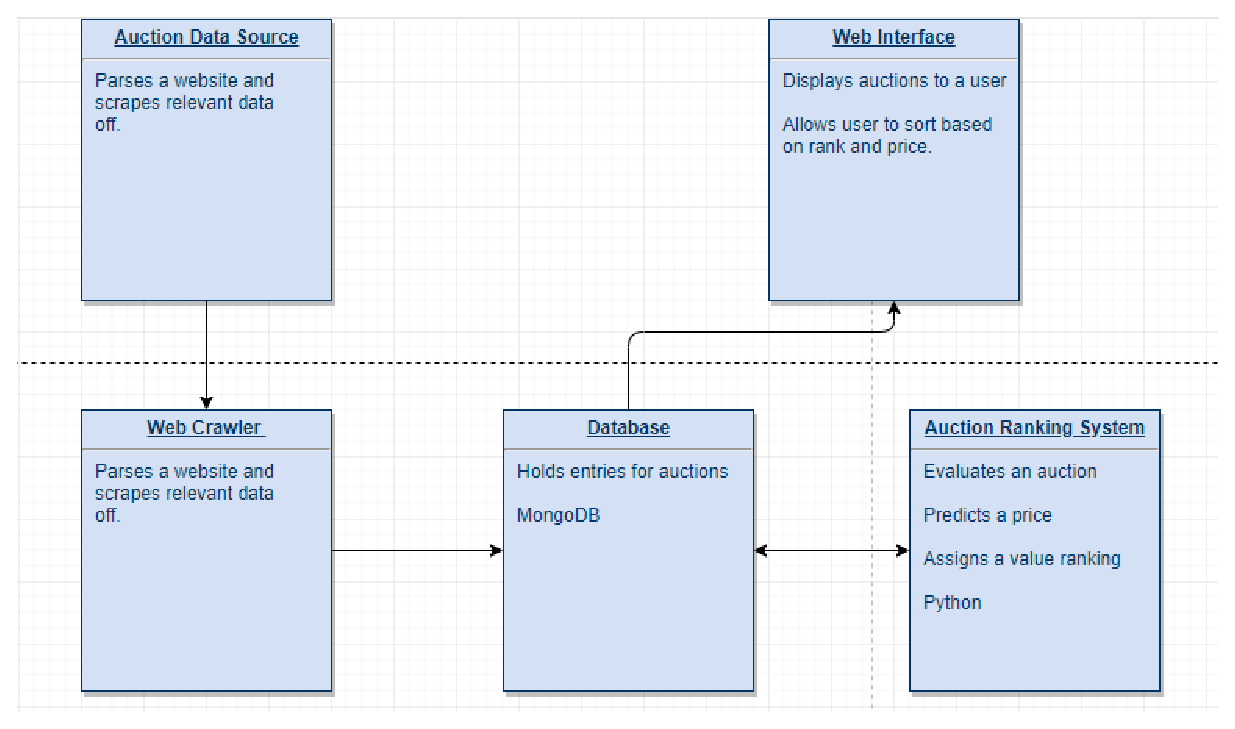
\includegraphics[scale=0.75]{flow_capture}
\caption{Flow Design}
\label{fig:flow}
\end{figure}

%-describes any problems that have impeded your progress, with any solutions you have,
\section{Obstacles}
The biggest obstacle that we have faced thus far is communication. This includes communication with out client, instructors, and TA. We were able to improve over the course of the term, but we should have been more proactive in the first few weeks. Our group never got far off track, so the impact was minimal. However, there were a few points that could have been made easier if we had better communication. 

Another obstacle was finding a way to arrive at a group decision on the choices of technology. Because the technology review was an individual assignment, we were unable to fully discuss the pros and cons of each choice with our team. In the end, our group is happy with the choices that were made individually. 

%-includes particularly interesting pieces of code (if coding is involved), and
\section{Interesting Code}  % again I don't think we have any code?
\subsection{MongoDB database}
Below is an example of how to create a new entry in Python using a MongoDB database \cite{mongoDB}. We can create a uniform auction entry template, then fill in relevant data that we pull from the website. Ideally we will modify this template to match 1:1 with all the important data that the auction websites provide. It may be the case that we don't end up using every piece of data, but it is important to not limit ourselves later down the pipeline. 
\begin{figure}[ht]

\begin{minted}{python}
db.inventory.insertOne(
   { item: "Tesla Model S", price: 12500, tags: ["bumper damage"] }
)
\end{minted}

\caption{MongoDB 'insert' example}
\end{figure}

Below is an example python call that can be made using MongoDB to find a particular subset of our database. In this example, we would find all entries with a price greater than \$10,000. This will be a crucial component when we go to implement our website UI and value calculation components.

\begin{figure}[ht]
\centering
\begin{minted}{python}
db.collection.find( { price: { gt: 10000 } } )
\end{minted}
\caption{MongoDB 'find' example}
\end{figure}



% Yufei: something pseudocode for web scrawler in Python
\subsection{Web Scraper}
When customers are trying to buy a salvage car and they will want to see the prices at different platforms at a single place. In such situations, Web crawler will full play its function on building an aggregator platform.

IAAAI.com is a website that sells salvage cars.\cite{IAAI} It will be our test site, and we are going to scrape Timed Auctions for salvage cars. The first step is to generate a basic spider using python:

\begin{minted}{python}
scrapy genspider timedauctions https://www.iaai.com/TimedAuctions
\end{minted}

That is what the IAAAI Timed Auctions page looks like:

\begin{figure}[ht]
\centering
\includegraphics[scale=0.5]{timedauctions}
\caption{Timed Auctions Page}
\label{fig:auction}
\end{figure}
\newpage
From this page, the following data about a salvage car needs to be extracted:

\begin{itemize}
\item Salvage car photo
\item Salvage car current bid
\item Salvage car VIN
\item Salvage car time remaining
\item Salvage car price
\end{itemize}

\textbf{Extracting the URLs include salvage car photo:}

After searching through the web page source code by using the developer tools of Chrome. We found that the car photos are stored under vis.iaai.com with imageKeys.

\begin{figure}[ht]
\centering
\includegraphics[scale=0.55]{salvagecarphoto}
\caption{Salvage Car Photo}
\label{fig:salvage}
\end{figure}

The attribute "imageKeys" can be used to extract image URLs. 
\begin{minted}{python}
response.css("img::attr(imageKeys)").extract()
\end{minted}
\newpage
\textbf{Extracting the URLs include salvage car current bid:}

We can use a similar method to find VIN's location which is an attribute of the \textless tbody\textgreater  tag.

\begin{figure}[ht]
\centering
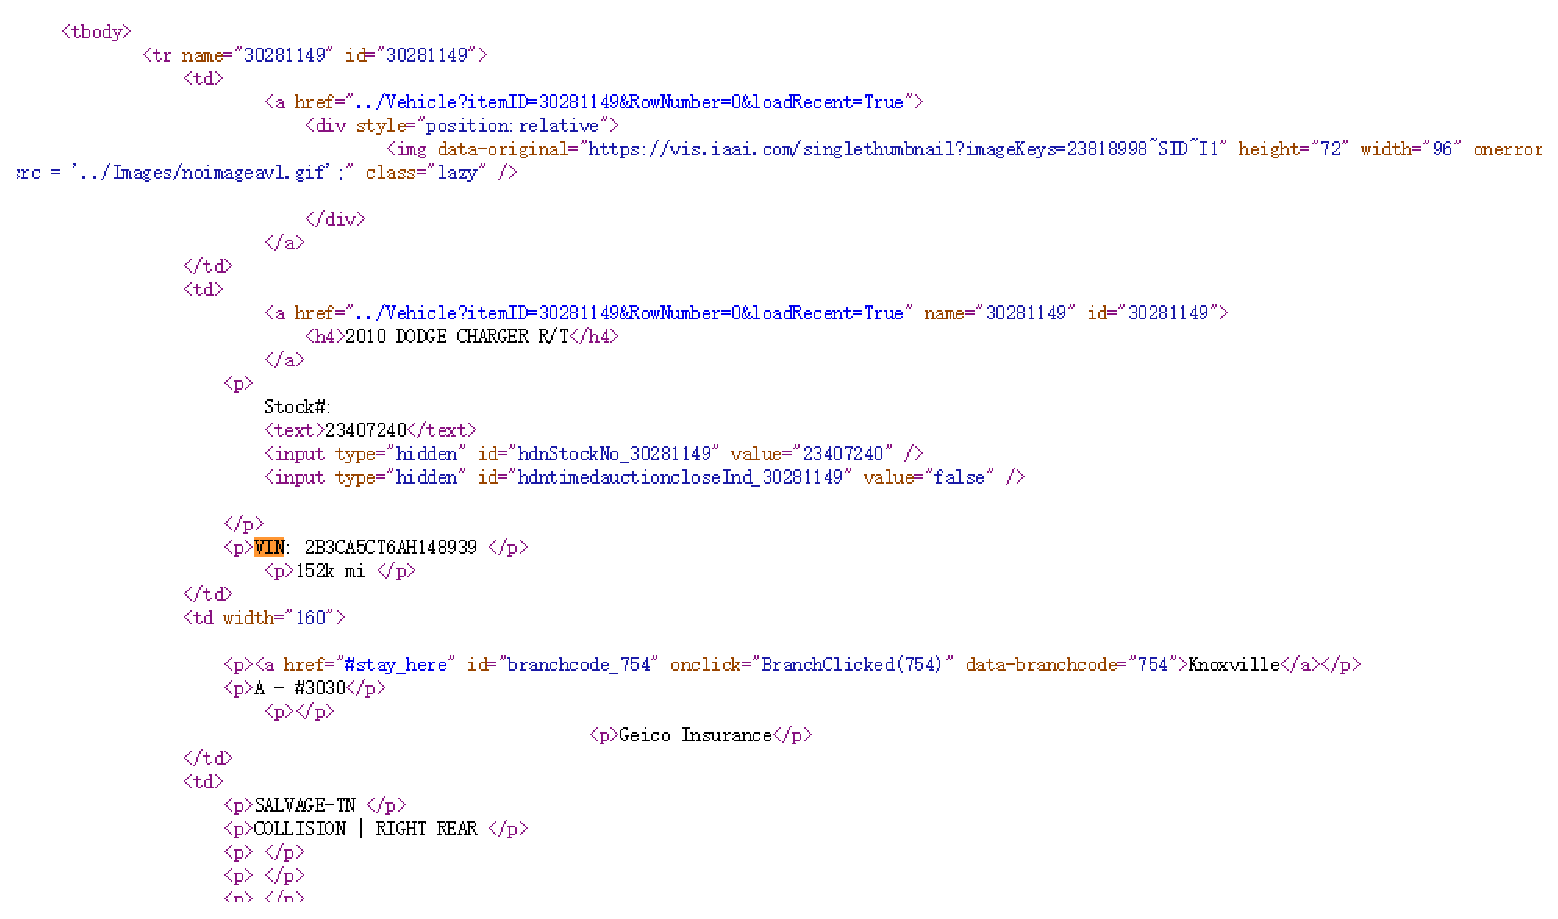
\includegraphics[scale=0.65]{salvagecarvin}
\caption{Salvage Vin Photo}
\label{fig:vin}
\end{figure}

%\centerline{
% 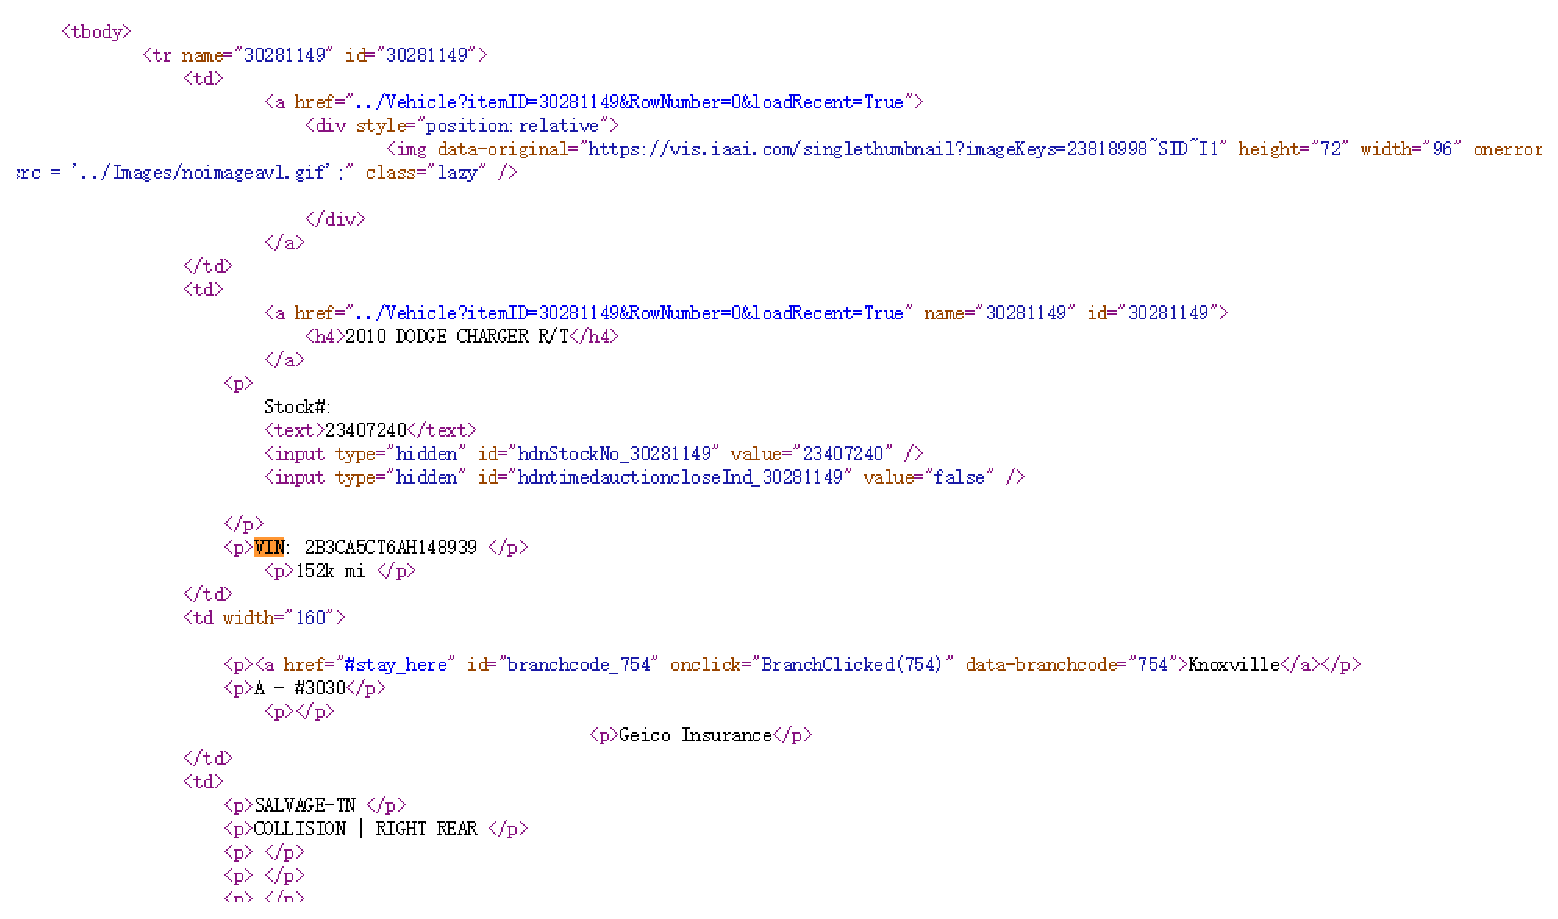
\includegraphics[width=80mm]{salvagecarvin}
% }

\begin{minted}{python}
response.css("tbody::attr(vin)").extract()
\end{minted}

\textbf{Extracting the URLs include salvage car remaining time and price:}

Similarly, we are able to extract the remaining time and price of salvage car.

\textbf{Time to download the extracted photos of salvage car:}

As mentioned in Design Document, Scrapy provides the images pipelines: once we got the data from website, we are able to pass them through different pipelines. By taking advantage of this function, the image pipeline allows us to download extracted photos of salvage car. In addition, we are able to convert the format of images and generate thumbnail.

\begin{minted}{python}
#enable the images pipeline.
SalvageCarPhotos_PIPELINES='scrapy.pipelines.images.ImagesPipeline': 1
#set the local download address.
Photo_Store = 'Users/Desktop/SalvageCarPhotos/'
\end{minted}

\begin{minted}{python}
#Generate two kinds of thumbnail for each salvage car photo, one small, one large.
GenerateThumbnail = {'small': (20, 20), 'large': (100, 100),}

\end{minted}




%-retrospective* of the past 10 weeks.
%-The document should include a detailed, week-by-week summary of activities, problems, solutions, and the like (consider using your blogs to inform this report). The report should not include more than a summary of any bigger documents you produced. 
\section{Retrospective}

% automatic row numbering
\newcounter{magicrownumbers}
\newcommand\rownumber{\stepcounter{magicrownumbers}\arabic{magicrownumbers}}
\begin{longtable}{ | c | *{3}{p{.3\linewidth} |} }
    \hline
    Week & Positives (What we completed) & Deltas (What we need to complete) & Actions (How we are going to complete them) \\ \hline
    % 1
    \rownumber & 
    Fictional Biography (individual assignment for self-introduction.), Resume (individual assignment for applying jobs or graduate school.)
    & We will individually need to complete the resume peer review. 
    & We all have partially finished resumes already, so it is a matter of updating.  \\ \hline
    
    % 2
    \rownumber & 
    Select a project (individual assignment.)
     & 
    We will individually need to decide on a project, and complete the project selection quiz. 
     & 
    We will be able to contact a number of clients to get in touch prior to the selection to see if the project is the right fit. 
    \\ \hline
    
    % 3
    \rownumber & 
    Problem Statement (individual assignment, including the details from client meeting and project proposal.)
    & 
    We plan to complete the group problem statement tonight. We also want to look into other forms of communication so my group can collaborate on a project at the same time while working remotely.
     & 
    For the time being we will use Discord for real time communication, and Slack for all other communication. 
     \\ \hline
    
    % 4
    \rownumber & 
    Group Problem Statement(group assignment, combining each group member's problem statement into one document.)
     & 
    We will need to start looking at the requirements document and work to get in better contact with our client. 
     & 
    We will make sure that our client is in our Slack channel so he will stay closer in the loop and we can have a place to ask questions. We will discuss some project details with our client to make sure we add them to the requirement document. 
     \\ \hline
    
    % 5
    \rownumber & 
    Our team has drafted up the majority of our requirements document. We are now waiting to hear back from our client to get some feedback and/or approval. 
     & 
   We plan to complete the requirements document this weekend, after we hear back from our client. 
     & 
     We have contacted our client over email, although we had the wrong address. We were able to resolve this over slack.
     \\ \hline
     
    % 6
    \rownumber & 
    Our group recently finished the requirements document. We collaborated well for this last assignment and things went well. Our group also got together and assigned portions of the project for the tech review.
     & 
    We will start looking at available technologies and begin testing.
     & 
    For each task that needs to be completed, we can look into sample code or technologies that could fulfill our requirements.
     \\ \hline
    
    % 7
    \rownumber & 
    Our group is working on applying all feedback from the tech review peer review.
     & 
    We are working on completing our final tech reviews.
     & 
    The combination of the two reviews will be used to edit our technology review drafts to work towards a final. The main points of concern are being less vague. 
     \\ \hline
    
    % 8
    \rownumber & 
    We have finished the technology review and agreed on the technologies to use. 
     & 
    We will need to learn more about the technologies that we chose, how to effectively use them, and putting the pieces together. 
     & 
    Looking at example code is a good place to start. Since our basic needs are fairly simple, we can research starter code to get an idea of what needs to be done. 
     \\ \hline
    
    % 9
    \rownumber & 
    We finished some initial technology investigation to see what the implementation would involve. We generated some code snippets. 
     & 
    We plan to begin working on the design document soon. 
     & 
    Since we are all celebrating the holiday weekend, we likely won't putting a lot of work into it until the Sunday. Thankfully there are large individual components that we can all think about before starting. 
     \\ \hline
     
    % 10
    \rownumber & 
     We finished the design document, and were able to pull information from our technology reviews. 
     & 
    Looking forward, the progress report and client verification still needs to be completed. 
     & 
    We agreed that we will all work on the written progress report, then copy a lot of the info to the presentation. To make recording easier, we will have two members create the presentation and one member speak over it. 
     \\ \hline
\end{longtable}

\bibliographystyle{IEEEtran}
\bibliography{IEEEabrv,bib}


\end{document}
